\documentclass[12pt]{extarticle}

\usepackage{amsmath, amsfonts, amsthm} % Math packages

\usepackage{listings} % Code listings, with syntax highlighting

\usepackage[main = greek, english]{babel} % English language hyphenation

\usepackage{graphicx} % Required for inserting images
\graphicspath{{Figures/}{./}} % Specifies where to look for included images (trailing slash required)

\usepackage{booktabs} % Required for better horizontal rules in tables

\usepackage{dirtytalk} % Required for quoting.

\usepackage{float} % Added for hard placement of images.

\usepackage[dvipsnames]{xcolor} % Added for extra colors.

\usepackage{tikz} % For colored boxes and more.

\numberwithin{equation}{section} % Number equations within sections (i.e. 1.1, 1.2, 2.1, 2.2 instead of 1, 2, 3, 4)
\numberwithin{figure}{section} % Number figures within sections (i.e. 1.1, 1.2, 2.1, 2.2 instead of 1, 2, 3, 4)
\numberwithin{table}{section} % Number tables within sections (i.e. 1.1, 1.2, 2.1, 2.2 instead of 1, 2, 3, 4)

\usepackage[utf8]{inputenc} % Required for inputting international characters
\usepackage[T1]{fontenc} % Use 8-bit encoding

\usepackage{translator}

\newcommand{\en}[1]{\foreignlanguage{english}{#1}}
\newcommand{\src}[1]{{\texttt\en{#1}}}


% Extra Formatting

\setlength{\parindent}{0em}
\setlength{\parskip}{0em}


% Code Listing Style

\lstdefinestyle{code}{
  belowcaptionskip=1\baselineskip,
  breaklines=true,
  frame=LRTB,
  xleftmargin=\parindent,
  showstringspaces=false,
  basicstyle=\ttfamily,
  keywordstyle=\bfseries\color{green!40!black},
  commentstyle=\itshape\color{purple!40!black},
  identifierstyle=\color{black},
  stringstyle=\color{orange},
}


\newcommand{\lstcode}[3]
{
    \begin{otherlanguage}{english}
    \lstinputlisting[language=#2, frame=single, style=code, caption=#3]{#1}
    \end{otherlanguage}
}

\usepackage{lineno}
\usepackage{hyperref}
\usepackage{cleveref}
\usepackage{epigraph} 
\modulolinenumbers[5]
\usepackage{caption}
\usepackage{subcaption}
\usepackage[margin=1in]{geometry}

\usetikzlibrary{positioning}
\usetikzlibrary{dsp,chains}

\DeclareMathAlphabet{\mathpzc}{OT1}{pzc}{m}{it}
\newcommand{\z}{\mathpzc{z}}

\crefname{equation}{εξ.}{εξ.}
\crefname{listing}{καταχώριση}{καταχώριση}

\makeindex

\bibliographystyle{ieeetr}

\newcommand{\filterspectrums}[2]
{
\begin{figure}
     \centering
     \begin{subfigure}[b]{\textwidth}
         \centering
         \includegraphics[width=\textwidth]{#1.png}
         \caption{Φασματογράφημα του τελικού αρχείου.}
     \end{subfigure}
     \hfill
     % \begin{subfigure}[b]{\textwidth}
     %     \centering
     %     \includegraphics[width=\textwidth]{#1_spectrum.png}
     %     \caption{Το φάσμα (πράσινο).}
     % \end{subfigure}
     \hfill
        \caption{#2}
        % \label{fig:sus}
\end{figure}
}

\begin{document}

\begin{titlepage}

\title{Σχεδιασμός και υλοποίηση ψηφιακού ισοσταθμιστή ήχου.}

%% Group authors per affiliation:
\author{Ευάγγελος Λάμπρου}
\date{}

\maketitle


\begin{abstract}
    Στα πλαίσια αυτής της εργασίας γίνεται ο σχεδιασμός και υλοποίηση 
    ενός ισοσταθμιστή ήχου. 
    Η ανάπτυξή του συστήματος ψηφιακής επεξεργασίας σήματος, όπως 
    και η γραφική διεπαφή έγιναν μέσα στο περιβάλλον του 
    \en{JUCE Framework} χρησιμοποιώντας τη γλώσσα \en{C++}. 
    Γίνεται η ανάλυση της θεωρίας πίσω από την ανάπτυξη των φίλτρων, 
    την υλοποίηση του συστήματος από το χαμηλό έως το υψηλό επίπεδο αφαιρετικότητας που 
    προσφέρει το πακέτο \en{JUCE}. 
    Τέλος, υπάρχει ανάλυση των επιδόσεων του φίλτρου όπως και μία σύντομη αναφορά πάνω 
    στην ευκολία χρήσης του.
    
    Η χρήση της συγκεκριμένης γλώσσας και βιβλιοθήκης έγινε με κριτήριο την ύπαρξη άφθονου
    εκπαιδευτικού υλικού πάνω σε αυτές τις τεχνολογίες και της άνεσής μας με αυτές. 
    Στην εργασία γίνεται προσπάθεια εστίασης στις βασικές έννοιες. Συνεπώς, πολλά από
    αυτά που θα αναφερθούν εφαρμόζονται και σε άλλα πακέτα ανάπτυξης \en{DSP} εργαλείων.

    Γίνεται ακόμα μία σύντομη παρουσίαση ανάπτυξης ενός \en{DSP plugin}. Πέραν από
    την ανάπτυξη του κώδικα υπεύθυνου για την ψηφικαή επεξεργασία ήχου, υφίσταται
    και ανάλυση του περιβάλλοντος μέσα στο οποίο θα υπάρχει αυτή η εφραμογή.

    Θα παραθέσουμε τα κύρια σημεία και θα δείξουμε τον τρόπο με τον οποίο
    κάποιος μπορεί να στήσει τώρα ένα σύστημα ικανό για περίπλοκη διαχείριση
    των πηγών ήχων του. 
\end{abstract}

\tableofcontents

\end{titlepage}

% \linenumbers

\section{Εισαγωγή}

\subsection{Στόχοι} 

Τελικός στόχος της εργασίας είναι η δημιουργία ενός ψηφιακού ισοσταθμιστή. 
Μία τέτοια εφαρμογή θα είναι ουσιαστικά υλοποίηση ενός ψηφιακού φίλτρου. 
Σαν είσοδο θα έχουμε διακριτές τιμές, δείγματα ήχου. 
Η επεξεργασία των σημάτων αυτών πρέπει να γίνεται σε πραγματικό χρόνο. 
Αυτή η ιδιότητα ίσως να μην είναι υποχρεωτική, εφόσων ο χρήστης 
θα μπορούσε απλά να εισάγει ένα αρχείο ήχου στο φίλτρο μας και να παίρνει ένα 
άλλο αρχείο πίσω. Τότε, ο χρόνος επεξεργασίας θα μπορούσε να είναι αρκετά 
μεγάλος (εντός λογικών ορίων). 
Ωστόσο, στόχος μας είναι η ανάπτυξη μιας εφαρμογής που θα μπορεί να χρησιμοποιηθεί 
εντός ενός περιβάλλοντος δημιουργίας μουσικής. Εκεί, η επεξεργασία του σήματος σε πραγματικό 
χρόνο είναι απαραίτητη μιας και ο χρήστης θα χρειάζεται να ακούει το αποτέλεσμα της επεξεργασίας
και να αλλάζει τα χαρακτηριστικά του φίλτρου ενώ δουλεύει.
Ο τρόπος με τον οποίο θα αλλάζουν οι ιδιότητες του φίλτρου είναι μέσω μίας γραφικής διεπαφής. 

\subsection{Αντίστοιχες Εφαρμογές}

Η ιδέα για την υλοποίηση ενός φίλτρου δεν είναι καινούρια. 
Στο σημείο αυτό θα κάνουμε μία σύντομη 
παρουσίαση μερικών άλλων \en{filter plugins} \footnote{
Όσα λογισμικά αναφερθούν είναι ανοιχτού κώδικα και είναι διαθέσιμα σε κάθε κύρια πλατφόρμα.
}, επισημαίνοντας ορισμένα τους 
αξιοσημείωτα χαρακτηριστικά.


\subsubsection{\en{LSP Parametric Equalizer}}

Η οικογένεια \en{plugins} των \en{LSP (Linux Studio PLugins)} είναι 
πολύ δημοφιλή στους κύκλους των μουσικών σε πλατφόρμες \en{GNU/Linux}. 
Στην περίπτωση αυτού του φίλτρου \cite{LSPEQ}, ο χρήστης έχει μπορστά του μία 
πολύ σύνθετη διεπαφή, μέσω της οποίας μπορεί να κόψει ή να αυξήσει συχνότητες σε 
16 διαφορετικά σημεία του φάσματος.
Ακόμα, υπάρχει οπτικοποίηση του σήματος
πριν και μετά το φίλτρο με \en{FFT}. Ακόμα, δίνεται 
η δυνατότητα επιλογής μεταξύ \en{IIR, FIR} φίλτρου.

Στόχος του \en{plugin} δεν είναι ο χρωματιστός του ήχου άλλα 
η διόρθωση του σήματος στο πεδίο της συχνότητας. Κάποιος μπορεί 
να επιλέξει το ακριβές είδος φιλτραρίσματος μεταξύ επιλογών 
όπως \en{Bell Filter, Resonance Filter, Billinear Transform Filter (BT), Match Z Transform (MZ) Filter} κ.α.
Στις οδηγίες χρήσης της εφαρμογής δίνονται οδηγίες σχετικά με σενάρια στα οποία υπερτερεί το κάθε 
είδος φίλτρου όταν εφαρμόζεται κατά την ισοστάθμιση.

\begin{figure}[!htb]
    \centering
    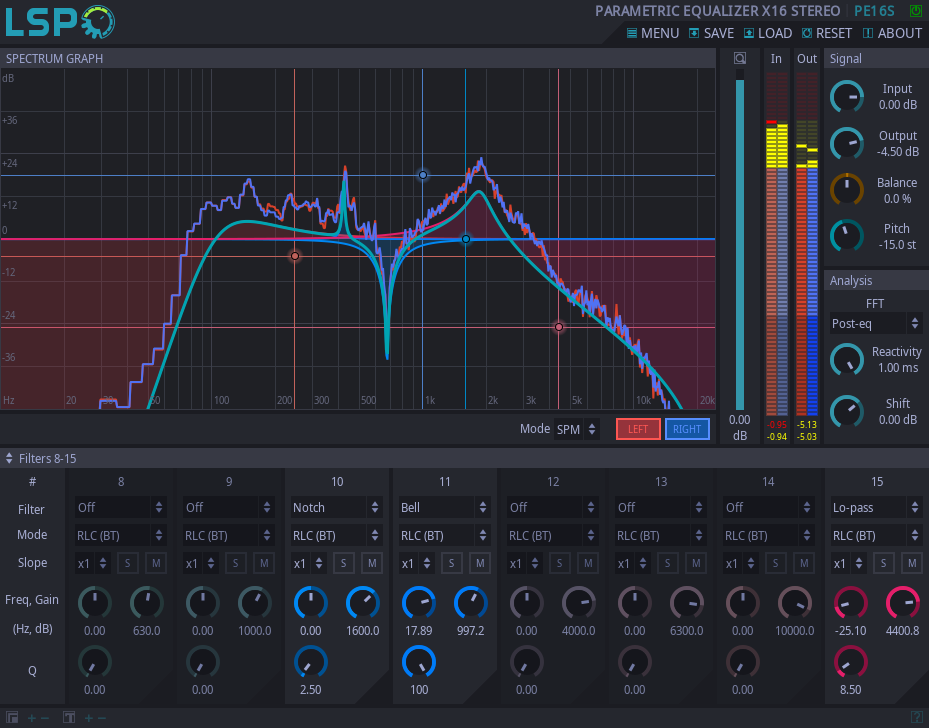
\includegraphics[width=.8\textwidth]{./assets/lsp_eq.png}
    \caption{Στιγμιότυπο του \en{LSP Parametric Equalizer}}
    \label{fig:}
\end{figure}

\subsubsection{\en{Calf Equalizer}}

Η οικογένεια των \en{Calf} \cite{Calf} \en{plugins} αποτελεί επίσης μία πολύ 
δημολιφής επιλογή στον κόσμο των \en{plugins} ανοιχτού κώδικα. 
Η γραφική διεπαφή κρατάει τα απαραίτητα ώστε να γίνει 
λεπτομερής επεξεργασία του φάσματος, χωρίς όμως να προσφέρει εξαντλητικές 
επιλογές. Ωστόσο, η πιο απλοϊκή εμφάνιση ίσως να το κάνει 
καταλληλότερο για καθημερινή χρήση στα πλαίσια παραγωγής μουσικής.

\begin{figure}[!htb]
    \centering
    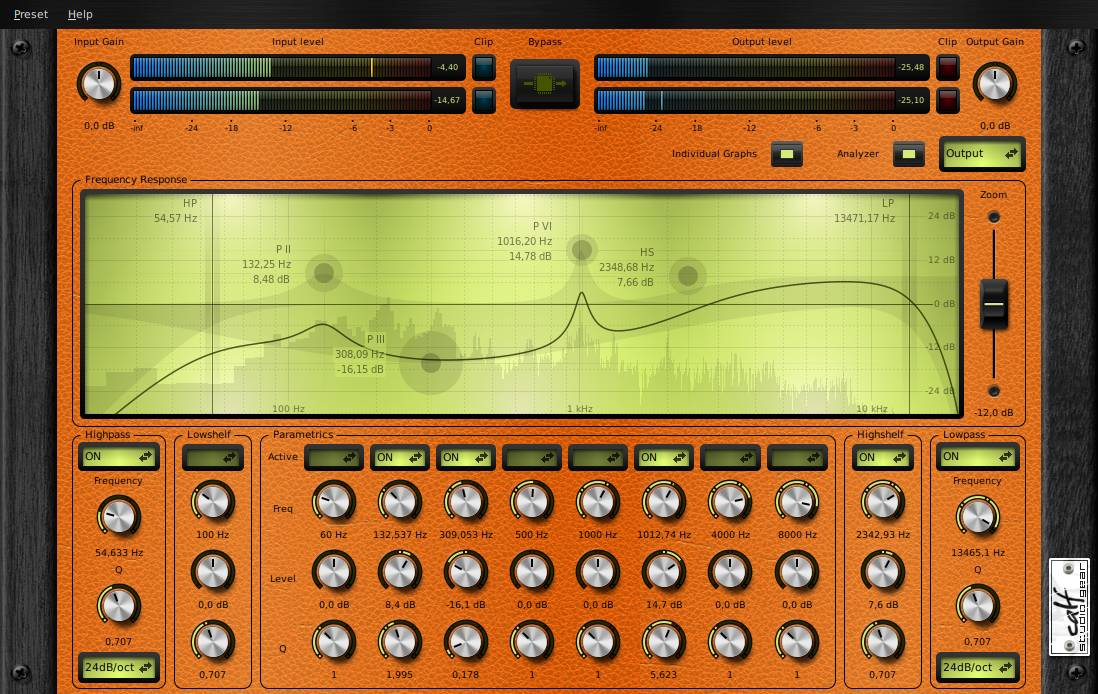
\includegraphics[width=0.8\textwidth]{./assets/calf.png}
    \caption{Στιγμιότυπο του \en{Calf Equalizer}}
    \label{fig:}
\end{figure}



\section{Σχεδιασμός}

\begin{figure}[!htb]

    \begin{center}
        \begin{tikzpicture}

        \node [draw,
        fill=Goldenrod,
        minimum width=2cm,
        minimum height=1.2cm,
        right=1cm
            ] (dsp) {$DSP$};

        \draw[->] ++(-1,0) -- (dsp.west) 
            node[midway,above]{$audio_{in}$};

        \draw[->] (dsp.east) --  ++(+2,0) 
            node[midway,above]{$audio_{out}$};
        \end{tikzpicture}
    \end{center}

    \caption{Βασική δομή του \en{plugin}.} 
\end{figure}

\subsection{Θεωρία \en{IIR} φίλτρων}

Στην εργασία αυτή θα περιοριστούμε στην υλοποίηση φίλτρων 2ης τάξης, με τους 
αλγόριθμους όμως να είναι ικανούς να παράγουν φίλτρα οσοδήποτε μεγάλης τάξης (χωρίς 
βέβαια να εγγυάται η ορθότητα του τελικού αποτελέσματος λόγω πεπαρασμένης ακρίβειας 
στις τιμές των συντελεστών). 

Έχοντας ως βάση ένα χαμηλοπερατό φίλτρο 2ης τάξης \cite{OpenheimAlan}

\begin{equation}
    H(s) = \frac{1}{s^2 + s/Q + 1} 
    \label{eq:h_lowpassfilter}
\end{equation}

Μέσω του διπολικού $Z$ μετασχηματισμού, θέτωντας $s = \frac{1}{K}\frac{z-1}{z+1} \; K = \frac{1}{2F_s}$ έχουμε \cite{BilinearZTransformWeb}

\begin{equation}
    H(z) = \frac{K^2 + 2K^2 z^{-1} + K^2 z^{-2}}{(K^2 + K/Q + 1) + 2(K^2 - 1) z^{-1} + (K^2 - K/Q + 1) z^{-2}}
    \label{eq:h_z_final}
\end{equation}


\subsection{Φίλτρα \en{Butteworth}} 

Επιλέξαμε το φίλτρο \en{Butterworth} σχεδόν αυθαίρετα. Ωστόσο, το φίλτρο 
έχει ορσιμένες ιδιότητες που το κάνουν θεμιτό στα πλαίσια επεξεργασίας ήχου.
Αρχικά, τα φίλτρα αυτά δεν έχουν \en{ripple} κοντά στη συχνότητα αποκοπής 
και έτσι δεν υπάρχει ενίσχυση καμίας συχνότητας. Ακόμα, 
έχουν πιο αργή αποκοπή ($-6n db/οκτάβα$, όπου $n$ η τάξη του φίλτρου). 
Αυτό σε εφαρμογές ήχου είναι πολλές φορές θεμιτό μιας και δίνει σαν αποτέλεσμα ένα πιο μαλακό 
κόψιμο των συχνοτήτων. Συνύθως δεν θέλουμε να διώξουμε ολοκληρωτικά τις αρμονικές 
από κάποιο όργανο.

\begin{figure}[!htb]
    \centering
    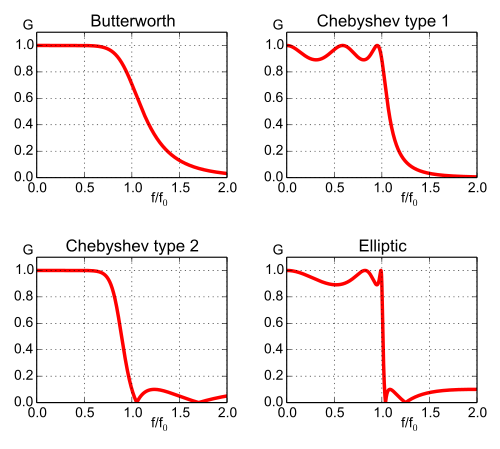
\includegraphics[width=0.8\textwidth]{./assets/comparison_filters.png}
    \caption{Σύγκριση φίλτρου \en{Butterworth} με άλλα φίλτρα.}
    \label{fig:}
\end{figure}

Για τους συντελεστές του φίλτρου \en{Butterworth} μπορούμε απλά να υπολογίσουμε την τιμή 
της σταθεράς $Q$ και να πάρουμε τους συντελεστές από την \cref{eq:h_lowpassfilter} \cite{OpenheimAlan, JuceDocumentation}

\begin{align}
    1/Q &= {2cos(\frac{2i + 1}{n}\pi)}, \; i = 0..\frac{n}{2} \qquad n = {\text{άρτιο}} \\ 
    1/Q &= {2cos(\frac{i + 1}{2n}\pi)}, \; i = 0..\frac{n}{2} \qquad n = {\text{περιττό}}
\end{align}

\subsubsection{Αλγόριθμος Υπολογισμού Συντελεστών}

Από την προηγούμενη μαθηματική ανάλυση, ο υπολογισμός των συντελεστών για το εκάστοτε φίλτρο είναι πλέον 
τετριμένος. 

Αντικαθιστώντας τις τιμές για το $Q$ για ένα φίτλρο \en{Butteworth} στη σχέση \ref{eq:h_z_final}
έχουμε πλέον τους συντελεστές του φίλτρου. 


\begin{align}
    a_0 &= \frac{K^2}{K^2 + K/Q +1} & a_1 &= 2a_0 & a_2 &= a_0 \\
    b_0 &= 1 & b_1 &= \frac{2(K^2 - 1)}{K^2 + K/Q + 1} & b_2 &= \frac{K^2 - K/Q + 1}{K^2 + K/Q + 1}
\end{align}

Ένα φίλτρο \en{Butteworth} 1ης τάξης έχει αποκοπή $-6dB/octave$, 2ης τάξης έχει αποκοπή $-12dB/octave$, ένα 3ης τάξης $-18dB/octave$ κοκ.

\section{Υλοποίηση}

\subsection{Βασική Αρχιτεκτονική}

Για την υλοποίηση του φίλτρου χρησιμοποιήθηκαν οι βιβλιοθήκες του πακέτου 
\en{Juce}. Το πακέτο αυτό χωρίζεται σε ενότητες \en{(modules)}, από τις οποίες
χρησιμοποιούμε κατά βάση την ενότητα \src{juce::dsp}. 
Εδώ, περιλαμβάνονται κλάσεις μέσω την οποίων μπορεί να γίνει η δημιουργία 
ενός φίλτρου.

Ο τρόπος με τον οποίο η εφαρμογή μας επεξεργάζεται τα εισερχόμενα δείγματα
\en{(samples)} είναι στη ρουτίνα \src{processBlock} όπου δεχόμαστε σαν είσοδο έναν
\en{buffer} από δείγματα στα οποία μπορούσαμε να εφαρφμόσουμε οποιονδήποτε αλγόριθμο. 

Το \en{plugin} στην πραγματικότητα αποτελείται από τρία (3) φίλτρα: 

\begin{enumerate}
    \item Ένα χαμηλοπερατό φίλτρο \en{(low pass filter)}
    \item Ένα φίλτρο κορυφής
    \item Ένα υψηπερατό φίλτρο
\end{enumerate}

\begin{figure}[!htb]

    \begin{center}

        \begin{tikzpicture}[node distance=3.0cm]

        % Controller

        \node [draw,
        fill=Purple,
        minimum width=1cm,
        minimum height=1.1cm,
            ] (lp) {$LP Filter$};

        \node [draw,
        fill=White,
        minimum width=1cm,
        minimum height=1.1cm,
        left of = lp
            ] (in) {$Source$};

        \node [draw,
        fill=Purple,
        minimum width=1cm,
        minimum height=1.1cm,
            ] (lp) {$LP Filter$};

        \node [draw,
        fill=Yellow,
        minimum width=1cm,
        minimum height=1.1cm,
            right of = lp] (pf) {$Peak Filter$};

        \node [draw,
        fill=Green,
        minimum width=1cm,
        minimum height=1.1cm,
            right of = pf] (hp) {$HP Filter$};

        \node [draw,
        fill=White,
        minimum width=1cm,
        minimum height=1.1cm,
        right of = hp
            ] (out) {$Output$};

        \draw[->] (in) -- (lp) 
            node[midway,above]{$audio_{in}$};
        \draw[->] (lp) --  (pf);
        \draw[->] (pf) --  (hp);

        \draw[->] (hp) -- (out) 
            node[midway,above]{$audio_{out}$};

        \end{tikzpicture}
    \end{center}

    \caption{Βασική δομή του \en{plugin}.} 
\end{figure}

Ο τρόπος με τον οποίο αυτό περιγράφεται στον κώδικα είναι μέσω της δομής 
\src{ProcessorChain} η οποία αναπαριστά μία αλυσιδά επεξεργαστών. 
Κατά την εκτέλεση της εφαρμογής, η ακολουθία από δείγματα
περνάει από την ρουτίνα επεξεργασίας του κάθε φίλτρου διαδοχικά. \cite{JuceDocumentation}

Στην περίπτωση που θέλαμε να έχουμε φίλτρο με πιο απότομη καμπύλη αποκοπής
συχνοτήτων (\en{slope}), θα μπορούσαμε να βάλουμε σε σειρά στο
\src{ProcessorChain} περισσότερα φίλτρα σε σειρά. Έτσι, ανάλογα με την καμπύλη
που θέλαμε θα μπορούσαμε να θέτουμε σε πέρασμα (\en{passthrough}) όλα τα
επίπεδα της αλυσίδας επεξεργασίας και να ενεργοποιούσαμε τον κατάλληλο αριθμό
από φίλτρα σε σειρά ανάλογα με το πόσο \say{απότομη} θα έπρεπε να είναι η καμπύλη.

Ο υπολογισμός της νέας αριθμητικής τιμής του κάθε δείγματος γίνεται με 
τη σειρά που φαίνεται στη \cref{fig:iir_filter_block}. 
Η καθυστέρηση του σήματος εισόδου γίνεται εφόσων το \en{plugin}
αποθηκεύει την κατάστασή του, η οποία είναι ένας πίνακας με τις τιμές της εξόδου 
του στα προηγούμενα δείγματα. Στην περίπτωση ενός φίλτρου 2ης τάξης 
αρκεί να αποθηκεύουμε τις δύο προηγούμενες τιμές εξόδου του.

\subsection{Επεξεργασία Δειγμάτων}

Η υλόποιση σε κώδικα όπως φαίνεται στην \cref{lst:iirimp} ταυτίζεται με τη σχηματική 
αναπαράσταση. Η βιβλιοθήκη \src{JUCE} έχει προνοήσει για τη χρήση τον ρουτίνων 
της με αριθμητικούς τύπους διαφορετικής ακρίβειας, εξού και η χρήση της 
λέξης-κλειδί \src{auto} \cite{CppReferenceAuto}, η οποία αναθέτει στον \en{compiler} το συμπέρασμα του τύπου 
της εκάστοτε μεταβλητής.

\begin{figure}
\centering
    \begin{tikzpicture}

	% Place nodes using a matrix
    \matrix (m1) [row sep=5mm, column sep=9mm]
    {
        \node[dspnodeopen, dsp/label=above] (x) {$x[n]$}     ; &
		\node[dspnodefull]                 (m11) {}          ; &
        \node[dspmixer, dsp/label=above]    (b0) {$b_0$}     ; &
        \node[dspadder]                     (adder) {}       ; &
		\node[coordinate]                   (m12) {}         ; &
		\node[dspnodefull]                   (m13) {}        ; &
        \node[dspnodeopen, dsp/label=above] (y) {$y[n]$}     ; &
        \\
        \node[coordinate]                   (mc) {}          ; &
		\node[dspsquare]                   (z01) {$\z^{-1}$} ; &
        \node[coordinate]                   (mc) {}          ; &
        \node[coordinate]                   (mc) {}          ; &
        \node[coordinate]                   (mc) {}          ; &
		\node[dspsquare]                   (z02) {$\z^{-1}$} ; &
        \\
        \node[coordinate]                   (mc) {}          ; &
        \node[dspnodefull]                   (m31) {}        ; &
        \node[dspmixer, dsp/label=above]    (b1) {$b_1$}     ; &
        \node[coordinate]                   (mc) {}          ; &
        \node[dspmixer, dsp/label=above]    (a1) {$-a_1$}    ; &
        \node[dspnodefull]                   (m32) {}        ; &
        \\
        \node[coordinate]                   (mc) {}          ; &
		\node[dspsquare]                   (z11) {$\z^{-1}$} ; &
        \node[coordinate]                   (mc) {}          ; &
        \node[coordinate]                   (mc) {}          ; &
        \node[coordinate]                   (mc) {}          ; &
		\node[dspsquare]                   (z12) {$\z^{-1}$} ; &
        \\
        \node[coordinate]                   (mc) {}          ; &
        \node[dspnodefull]                   (m51) {}        ; &
        \node[dspmixer, dsp/label=above]    (b2) {$b_2$}     ; &
        \node[coordinate]                   (mc) {}          ; &
        \node[dspmixer, dsp/label=above]    (a2) {$-a_2$}    ; &
        \node[dspnodefull]                   (m52) {}        ; &
        \\
    }                                                        ;

	% Draw connections

	\begin{scope}[start chain]
		\chainin (x);
		\chainin (m11) [join=by dspline];
		\chainin (b0) [join=by dspline];
		\chainin (adder) [join=by dspconn];
		\chainin (m13) [join=by dspconn];
		\chainin (y) [join=by dspconn];
	\end{scope}

	\begin{scope}[start chain]
		\chainin (m11);
		\chainin (z01) [join=by dspconn];
		\chainin (m31) [join=by dspconn];
		\chainin (b1) [join=by dspconn];
		\chainin (adder) [join=by dspconn];
	\end{scope}

	\begin{scope}[start chain]
		\chainin (m31);
		\chainin (z11) [join=by dspconn];
		\chainin (m51) [join=by dspconn];
		\chainin (b2) [join=by dspconn];
		\chainin (adder) [join=by dspconn];
	\end{scope}

	\begin{scope}[start chain]
		\chainin (m13);
		\chainin (z02) [join=by dspconn];
		\chainin (m32) [join=by dspconn];
		\chainin (a1) [join=by dspconn];
		\chainin (adder) [join=by dspconn];
	\end{scope}

	\begin{scope}[start chain]
		\chainin (m32);
		\chainin (z12) [join=by dspconn];
		\chainin (m52) [join=by dspconn];
		\chainin (a2) [join=by dspconn];
		\chainin (adder) [join=by dspconn];
	\end{scope}
	
\end{tikzpicture}


\caption{Υλοποίηση του \en{IIR} φίλτρου}
\label{fig:iir_filter_block}

\end{figure}

\begin{minipage}{\textwidth}
    \lstcode[lst:iirimp]{./assets/src/iir.cpp}{C++}{Ο υπολογισμός της νέας τιμής για το κάθε δείγμα σε \src{C++}}
\end{minipage}

Αξίζει να σημειωθεί πως στον πυρήνα του ένα οποιοδήποτε \en{plugin} επεξεργασίας 
ήχου είναι είναι ένα σύνολο από προσθέσεις, πολλαπλασιασμούς και καθυστερήσεις. 
Σε γενικές γραμμές, η υλοποίηση των περισσότερων 
αλγορίθμων δεν είναι αξιοσημείωτη, περά από πιθανές βελτιστοποιήσεις με τη χρήση παραλληλισμού. 

Σαφώς, βιβλιοθήκες όπως η \en{JUCE} φροντίζουν στην καλύτερη δυνατή υλοποίηση, 
αφού δεν υπάρχουν κατά το δυνατόν περιτές πράξεις και γίνεται προσπάθεια 
στη βελτιστοποίηση του κώδικα από τη φάση της μετάφρασης (\en{compilation}).

\paragraph{Γραφική Διεπαφή}

\epigraph{\en{The first 90 percent of the code accounts for the first 90 percent of
the development time. The remaining 10 percent of the code accounts for the
other 90 percent of the development time}}{\en{\textit{Tom Cargill, Bell Labs}}}

Η βιβλιοθήκη \en{JUCE} παρέχει τη δυνανότητα να αναπτύξει ο χρήστης 
σύνθετες γραφικές διεπαφές μέσα από τις οποίες μπορεί κάποιος να ελέγχει 
το \en{DSP} μέρος της εφαρμογής (συχνότητες αποκοπής κτλ).

Η βιβλιοθήκη \en{JUCE} επιτρέπει την δημιουργία διεπαφών 
ανεξάρτητες από την πλατφόρμα στην οποία θα εκτελεστεί η εφαρμογή. 
Ο κώδικας δημιουργίας παραθύρων και γραφικών είναι πολύ εξαρτούμενος από 
το σύστημα του χρήστη. Για αυτό η το λόγο προτιμείται να χρησιμοποιούνται 
τα εργαλεία της βιβλιοθήκης τα οποία παρουσιάζουν ένα \en{API} 
με το οποίο μπορούμε να δημιουργήσουμε μία διεπαφή αδιαφορώντας από την 
\en{low-level} επικοινωνία με το σύστημα του χρήστη.


\tikzset{
    block/.style={
        draw,
        inner sep=1pt,
        minimum width=2cm,
        minimum height=1.2cm,
        },
}

\begin{figure}[!htb]
    \centering
    \begin{tikzpicture}[node distance = 1.5cm]
        \node[block, fill=Goldenrod] (system1) {\en{Windows Graphics API}};
        \node[block, fill=Goldenrod, below of = system1] (system2) {\en{Linux Graphics API}};
        \node[block, fill=Goldenrod, below of = system2] (system3) {\en{Other Graphics API}};
        \node[block, fill=SkyBlue, right=2cm of system2] (juce) {\en{JUCE Graphics API}};
        \node[block, fill=Green, right=2cm of juce] (code) {\en{Plugin Code}};

        \foreach \sys in {system1, system2, system3}
        {
            \draw[line width=1, -] (juce) -- (\sys.east) node[]{};
        }

        \draw[line width=1, -] (code) -- (juce) node[]{};
    \end{tikzpicture}
    \caption{Χρήση του \en{API} για γραφικά της βιβλιοθήκης \en{JUCE}}
\end{figure}

Έτσι, μπορούμε να γράψουμε τον κώδικα για γραφικά μία φορά και 
να λειτουργεί σε όλες τις πλατφόρμες.

Είναι άξιο αναφοράς πως σε γραμμές κώδικα, η γραφική διεπαφή χρειάστηκε 
περισσότερη συγγραφή σε σχέση με τον επεξεργαστή συμάτων. 
Αυτό δεν είναι βέβαια σίγουρο αν είναι πρωτέρημα ή όχι της βιβλιοθήκης.

Η τελική παρουσίαση των γραφικών στην περίπτωση του δικού μας συστήματος
γίνεται από το σύστημα παραθύρων (\en{windowing system}), ένα επίπεδο αφαίρεσης
το οποίο έχει πολλές αντιστοιχίες με τον \en{audio server}. Τα διαγράμματα \cite{XWindowWebsite}
αναφέρονται σε σύστημα \en{Linux} στο οποίο τρέχει το λογισμικό \en{X Server}. \cite{XWiki}
Ωστόσο, αρχιτεκτονική αυτή μπορεί να αντιστοιχεί σε οποιοδήποτε σύστημα.

\begin{figure}[h]
    \centering
    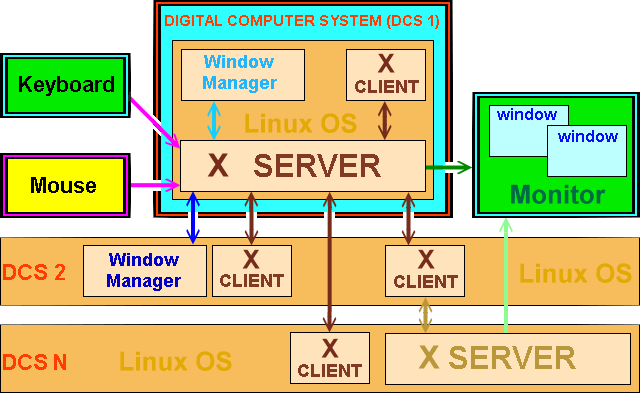
\includegraphics[width=0.8\textwidth]{./assets/xserver.png}
    \caption{Βασική αρχιτεκτονική \en{server-client} για το \en{X Window System}.}
    \label{fig:}
\end{figure}

Όλη η επικοινωνία μεταξύ του \en{plugin} και του συστήματος 
παραθύρων έχει \say{κρυφτεί} πίσω από ενός απλού \en{API} 
δημιουργίας γραφικών στοιχείων. Ακόμα και η δημιουργία 
του παραθύρου γίνεται αυτόματα από τη βιβλιοθήκη \en{JUCE}.

\begin{figure}[!htb]
    \centering
    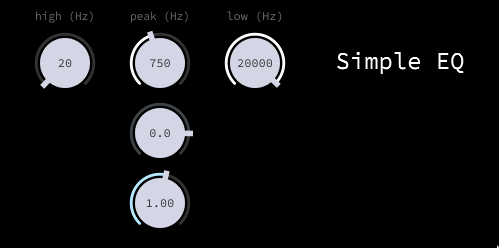
\includegraphics[width=0.8\textwidth]{./assets/GUI.png}
    \caption{Η τελική γραφική διεπαφή του ισοσταθμιστή.}
    \label{fig:finalgui}
\end{figure}

Στην τελική εφαρμογή υπάρχουν πέντε \en{knobs}:

\begin{itemize}
    \item Δύο για τον έλεγχο του υψιπερατού και του χαμηλοπερατού φίλτρου.
    \item Τρία για την επιλογή της \en{peak} συχνότητας, του \en{gain} το οποίο θα λάβει και του πάχους της καμπύλης, αντίστοιχα.
\end{itemize}

Ο έλεγχος του \en{DSP} μέσω της διεπαφής γίνεται μέσα από την ανταλαγή μυνημάτων 
που προκύπτουν από συμβάντα \en{events} \cite{EventsArchWiki}. Αυτού του είδους η αρχιτεκτονική 
είναι συνήθης σε πολλές βιβλιοθήκες ανάπτυξης διεπαφών.

\section{Χρήση}

\subsection{\en{Audio Plugin Hosts}}

Πλέον, η χρήση των περισσότερων εφαρμογών \en{DSP} γίνεται μέσα 
από άλλα προγράμματα τα οποία παίζουν το ρόλο του οικοδεσπότη 
και φιλοξενούν το δικό μας λογισμικό. Η επικοινωνία μεταξύ 
του \en{plugin} μας και του \en{host} γίνεται μέσα από 
ένα \en{API}, μέσα από το οποίο έχουν οριστεί οι δομές δεδομένων 
και οι ρουτίνες με βάση τις οποίες θα γίνει η μεταφορά πληροφορίας 
μεταξύ των δύο. 


Αυτή η επικοινωνία μπορεί να γίνει μέσα από το δυναμικό 
φόρτωμα κώδικα \cite{DynamicLoadWiki}, όπου 
ο κώδικας του \en{plugin} μας φορτώνεται και εκτελείται όσο τρέχει
το \en{host} πρόγραμμα. \cite{DesignPlugins}

Οι \en{hosts} συνοδεύονται συχνά από γραφικές διεπαφές και επιτρέπουν ακόμα 
το χειρισμό των \en{client} προγραμμάτων μέσα από τις δικές του γραφικές 
διεπαφές. Αυτή η επικοινωνία καθοδηγείται επίσης από ένα \en{API}. 

\begin{figure}[!htb]
    \centering
    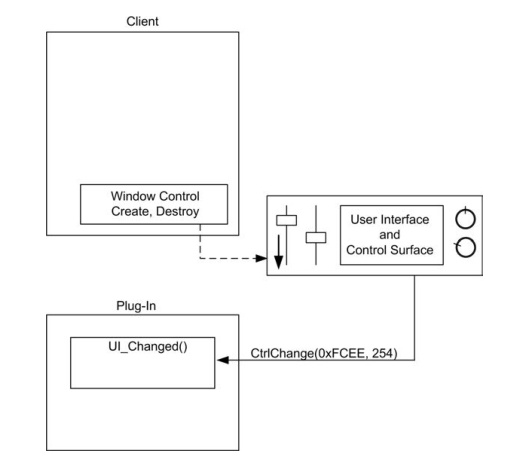
\includegraphics[width=0.8\textwidth]{./assets/plugin_client.png}
    \caption{Περίπτωση όπου ο \en{host} ελέγχει το \en{UI} το οποίο με τη σειρά του ελέγχει το \en{plugin}}
    \label{fig:}
\end{figure}

Το βασικό σημείο είναι η επξεργασία των δεδομένων ήχου. Εδώ, 
ο \en{audio plugin host} παίρνει σαν είσοδο τα δεδομένα ήχου (πχ. από τον σκληρό δίσκο) 
και τα προωθεί στο \en{plugin} που φιλοξενεί, μαζί με δεδομένα όπως 
το \en{sample rate} και ο αριθμός καναλιών.
Με τη σειρά του το \en{plugin} εκτελεί προκαθορισμένες ρουτίνες με βάση το \en{API}
στις οποίες εμείς έχουμε προσθέσει τον εξειδικευμένο κώδικά μας για την εφαρμογή μας.

\begin{figure}[!htb]
    \centering
    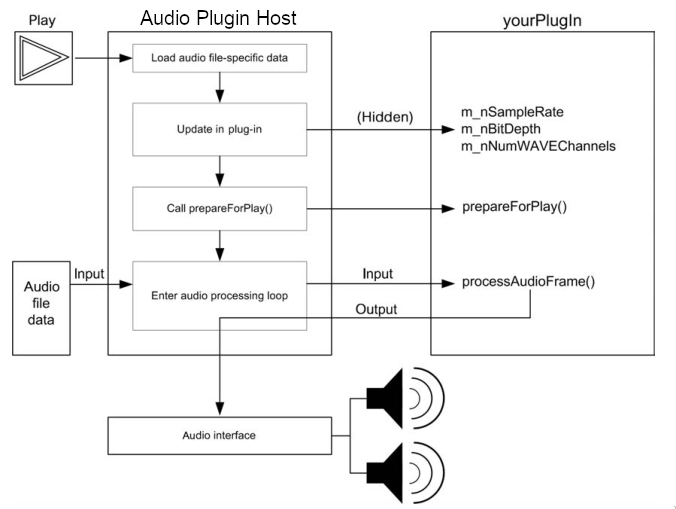
\includegraphics[width=\textwidth]{./assets/events.png}
    \caption{Η επικοινωνία μεταξύ του \en{Plugin Host} και του \en{Plugin} μας.}
\end{figure}

\begin{figure}[!htb]

    \begin{center}
        \begin{tikzpicture}[node distance = 2cm]

        \node [draw,
        fill=Goldenrod,
        minimum width=2cm,
        minimum height=1.2cm,
        ] (kernel) {\en{Kernel}};

        \node [draw,
        fill=GreenYellow,
        minimum width=2cm,
        minimum height=1.2cm,
        below of = kernel
        ] (sounddriver) {\en{Sound Card Driver}};

        \node [draw,
        fill=Thistle,
        minimum width=2cm,
        minimum height=1.2cm,
        right=2cm,
        right of = sounddriver
        ] (audioserver) {\en{Audio Server}};

        \node [draw,
        fill=Peach,
        minimum width=2cm,
        minimum height=1.2cm,
        right=2cm,
        right of = audioserver
        ] (app1) {\en{App}};

        \node [draw,
        fill=Peach,
        minimum width=2cm,
        minimum height=1.2cm,
        above of = app1
        ] (app2) {\en{App}};

        \node [draw,
        fill=Peach,
        minimum width=2cm,
        minimum height=1.2cm,
        below of = app1
        ] (app3) {\en{App}};

        \draw[->, line width =1] (sounddriver) -- (kernel) 
            node[midway,above]{};

        \draw[->, line width =1] (sounddriver) -- (audioserver) 
            node[midway,above]{};

            \foreach \app in {app1, app2, app3}
            {
                \draw[<->, line width =1] (audioserver) -- (\app) 
                    node[midway,above]{};
            }

        \end{tikzpicture}
    \end{center}

    \caption{Στοίβα τεχνολογιών ήχου σε ένα \en{Linux} σύστημα.} 
\end{figure}

\begin{figure}[!h]
    \centering
    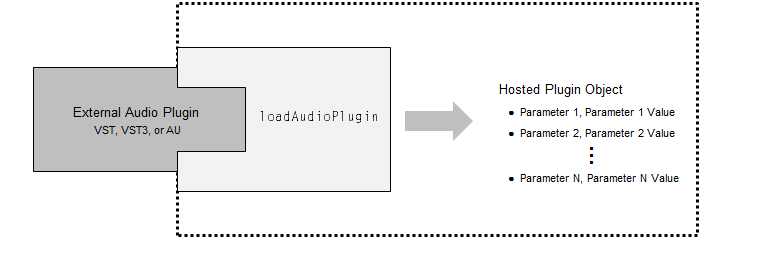
\includegraphics[width=\textwidth]{./assets/audio_plugin_host.png}
    \caption{Διάγραμμα ενός \en{audio plugin host}.}
    \label{fig:}
\end{figure}

\begin{figure}[!htb]
    \centering
    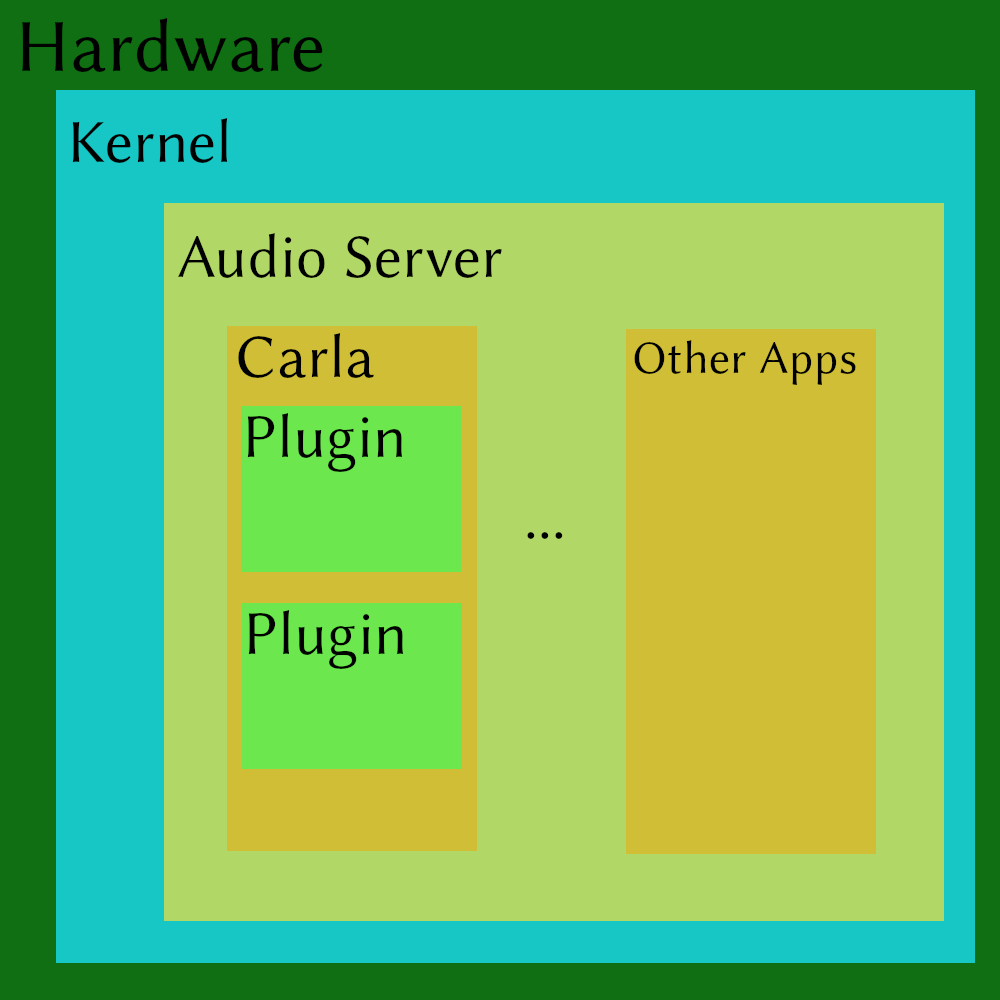
\includegraphics[width=\textwidth]{./assets/insides.png}
    \caption{Το περιβάλλον \en{Carla} επικοινωνεί με τον \en{audio server}, είναι μία από τις εφαρμογές του και ταυτόχρονα μπορεί να φιλοξενήσει άλλες εφαρμογές σαν \en{plugins}.}
\end{figure}



\subsection{Αρχιτεκτονική ήχου σε \en{Linux} σύστημα}

Πλέον, το πιο συνήθες σύστημα για \en{audio driver} έιναι το \src{ALSA}. \cite{ALSA} 
Αυτό με το οποίο, όμως, ένας χρήστης θα έρχεται περισσότερο σε επαφή
είναι ο διακοσμιτής ήχου (\en{audio server}). Αυτός βρίσκεται σε άμεση
επικοινωνία με τους \en{drivers} οι οποίοι τελικά θα πουν στο υλικό πώς να
συμπεριφερθεί ώστε να ακουστεί ήχος από μία συσκευή. Ο διακοσμιτής δέχεται
δεδομένα ήχου από πολλές διαφορετικές εφαρμογές και βγάζει μία ενιαία σειρά από
δεδομένα (\en{data stream}). Αυτό μας επιτρέπει να ακούμε πολλές ερφαρμογές ταυτόχρονα παιρνώντας
την καθεμία από το κανάλι ενός εικονικού \en{mixer}. Φυσικά, θα μπορούσαμε να
μην έχουμε έναν \en{audio server} και να επικοινωνούσε η οποιαδήποτε διεργασία
μας που παρήγαγε ήχο άμεσα με τον \en{driver}. Αυτό θα σήμαινε όμως πως μόνο μία
διεργασία θα μπορούσε να μιλήσει με την κάρτα ήχου ανά πάσα στιγμή, δεδομένου
το πώς είναι δομημένο το \en{audio backend} στο σύστημά μας. 
Αυτό βέβαια σε σημερινά δεδομένα είναι ανεπίτρεπτο, αφού ένα χρήστης πιθανότατα να χρειάζεται 
να ακούει ήχο ο οποίος προέρχεται από πολλές διαφορετικές εφαρμογές. Ακόμα και αν οι εφαρμογές 
αυτές δεν παράγουν ήχο ταυτόχρονα, η αντιστοίχιση της κάθε ροής σε ξεχωριστό κανάλι μας δίνει 
τη δυνατότητα να ελέγχουμε την ένταση (και ίσως άλλα χαρακτηριστικά) του ήχου που προέρχεται 
από τις διεργασίες μας ξεχωριστά. Αυτό μπορεί να συνδυαστεί με το σύστημά μας να έχει μνήμη 
με τις ρυθμίσεις μας για το κάθε κανάλι του ψηφιακού μίξερ, έχωντας έτσι διαφορετική 
ένταση ανάλογα με την εφαρμογή χωρίς να χρειάζεται ο χρήστης να επαναρυθμίζει την ένταση 
του εξοπλισμού του για την κάθε διαφορετική εφαρμογή.

Τώρα, για τον \en{audio server} υπάρχουν διάφορες επιλογές. Για πολύ καιρό η
βασική επιλογή ήταν το \en{PulseAudio} \cite{PulseAudio}, το οποίο 
κέρδισε έδαφος για την ευχρηστεία του, τις ποικίλες δυνατότητες που πρόσφερε μέσω 
\en{plugins} που μπορούσαν να φορτωθούν αλλά κυρίως με την συμβατότητα του με πολλά συστήματα.
Ωστόσο, είναι
αδύναμο σε εφαρμογές χαμηλής καθυστέρησης όπως είναι η παραγωγή μουσικής. Σε
αυτές τις περιπτώσεις χρησιμοποιείται ο διακοσμιτής \en{JACK} \cite{JACK}, 
ο οποίος αν και εύχρηστος απαιτεί περισσότερες τεχνικές γνώσεις για την αιξιοποίησή του.
Υπάρχει πλέον προσπάθεια δημιουργίας μίας νέα υλοποίησης η οποία θα
συμπεριλαμβάνει τα θετικά και των δύο \en{audio servers}. Αυτό είναι το
\en{Pipewire} \cite{Pipewire} και δίνει τη δυνατότητα εύκολης επικοινωνίας
μεταξύ όλων των συσκευών και διεργασιών του συστήματος, ακόμα και σε
περιβάλλοντα υψηλών επιδόσεων. Η μηχανή του \en{Pipewire} γίνεται
ευρέως αποδεκτή στην κοινότητα ακόμα και από τους προγραμματιστές των
\say{αντίπαλων} \en{audio servers}. \cite{PipewireLWNArt}

\subsection{Περιβάλλον Χρήσης \en{Plugin}}

\paragraph{\en{Carla}}

Για την χρήση του \en{plugin} \src{Simple EQ} μπορεί να γίνει 
σύνδεσή του με άλλες ροές ήχου στον υπολογιστή μέσω ενός \en{audio plugin host}.
Ένα πολύ ικανό και δημοφιλές είναι το λογισμικό \en{Carla} \cite{CarlaApp}, 
μέσα από το οποίο μπορούμε να κατευθύνουμε τη ροή ήχου από μία εφαρμογή 
στον υπολογιστή μας, μέσα από κάποιο \en{plugin} και τελικά να έχουμε την έξοδο 
στα ηχεία (ή οποιαδήποτε άλλη συσκευή).

Για να γίνει πιο κατανοητός ο τρόπος με τον οποίο 
το λογισμικό \en{Carla} παίρνει θέση ανάμεσα στις άλλες τεχνολογίες 
που χρησιμοποιούμε, μπορούμε να το φανταστούμε σαν ένα μεσάζοντα μεταξύ του 
\en{audio server} (\en{Pipewire}) και του \en{plugin} μας.

Η εφαρμογή \en{Carla} \say{κουμπώνει} στον \en{audio server} 
ή στον εγχώριο \en{sound driver}. Έτσι, μπορεί να ελέγχει την 
πορεία των σημάτων ήχου. Στην γραφική της διεπαφή ( \cref{fig:carla_basic} ) 
το μπλε χρώμα υποδηλώνει μία είσοδο/έξοδο \en{audio}, ενώ 
το κόκκινο χρώμα αντιστοιχεί σε μία είσοδο/έξοδο 
που χειρίζεται συμβάντα. Αυτά συνύθως αποτελούν \en{MIDI events}.

\begin{figure}[!h]
    \centering
    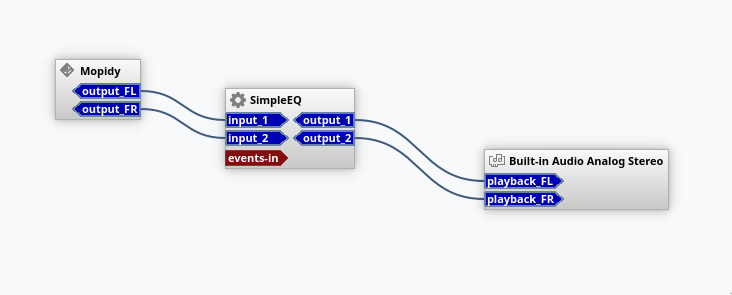
\includegraphics[width=0.8\textwidth]{./assets/Carla_Basic.png}
    \caption{Εφαρμογή του \src{SimpleEq plugin} στο περιβάλλον \en{Carla}.}
    \label{fig:carla_basic}
\end{figure}


\paragraph{\en{Digital Audio Workstation}}
Συνήθης είναι επίσης η χρήση του \en{plugin} μέσα από ένα λογισμικό 
\en{DAW (Digital Audio Workstation)}, όπου μπορούμε να φορτώσουμε δυναμικά 
το \src{Simple EQ}, να προσθέσουμε σε ένα από τα κομμάτια του \en{mixer} 
και έτσι όποιος ήχος περνάει σε εκείνο το κανάλι θα επεξεργάζεται από τον \en{plugin}. 

Η βιβιοθήκη \src{JUCE} προσφέρει συστήματα για το χτήσιμο (\en{build}) του κώδικα 
ως \en{plugin (VST3)} \cite{VSTWiki}, ή ως αυτόνομη εφαρμογή.  

\section{Μετρήσεις}

Μετά τη δημιουργία της εφαρμογής ισοστάθμισης, έγινε εισαγωγή του \en{plugin} 
\src{SimpleEQ} στο ψηφιακό περιβάλλον επεξεργασίας ήχου (\en{DAW}) \en{Ardour}, 
το οποίο λειτουργεί σαν υποδοχέας και παρέχει δυνατότητες μέτρησης της απόκρισης συχνότας και 
φάσης του φίλτρου (\cref{fig:ardour_analysis}).

\begin{figure}[!h]
    \centering
    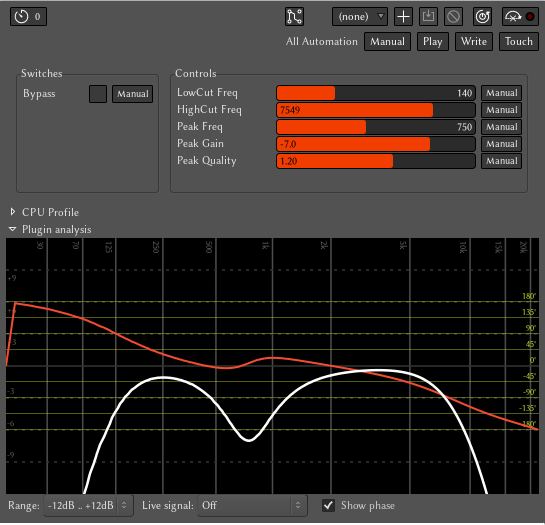
\includegraphics[width=0.8\textwidth]{./assets/PluginAnalysisArdour.png}
    \caption{Ανάλυση του \src{SimpleEQ} μέσα από το \en{Ardour}. Φαίνεται η απόκριση συχνότητας (άσπρο) και η απόκριση φάσης (κόκκινο).}
    \label{fig:ardour_analysis}
\end{figure}

Γίνεται φανερό από την απόκριση του φίλτρου πως η αποκοπή 
είναι \say{μαλακή} (\en{soft-cut}). 

\subsection{Μετρήσεις με \en{White Noise}}
Έπειτα, εφαρμόσαμε λευκό θόρυβο και αναλύσαμε το τελικό αρχείο ήχου.

\filterspectrums{./assets/WhiteNoise}{Το σήμα λευκού θορύβου χωρίς φίλτρο.}
\filterspectrums{./assets/WhiteNoiseLP}{Το σήμα λευκού θορύβου με εφαρμογή χαμηλοπερατού φίλτρου στα $1000Hz$.}
\filterspectrums{./assets/WhiteNoiseHP}{Το σήμα λευκού θορύβου με εφαρμογή υψιπερατού φίλτρου στα $1000Hz$.}

Μία παρατήρηση είναι πως στην περίπτωση του υψιπερατού φίλτρου, οι υψηλές συχνότητες φαίνεται 
να ενισχύονται παραπάνω από τα αρχικά τους επίπεδα. Αυτό πιθανότατα να οφείλεται στο αναπόφευκτο \en{phase shift}
που προκαλεί το \en{plugin} το οποίο προκαλεί συχνότητες να συγχρονιστούν σε φάση οδηγώντας σε διακρότημα
και έτσι ενίσχυσή τους.

\subsection{Μετρήσεις με πιο σύνθετα αρχεία}
Για μερικές ακόμα μετρήσεις χρησιμοποιήθηκε το τραγούδι \en{Bring Me the Disco King - David Bowie} 
το οποίο περάσαμε μέσα από \src{Simple EQ}. 

Όλα τα αρχεία τα οποία μελετάμε είναι κωδικοποιημένα σε μορφή \en{WAV 16-bit} με συχνότητα δειγματοληψίας $48kHz$.

\begin{figure}[!h]
    \centering
    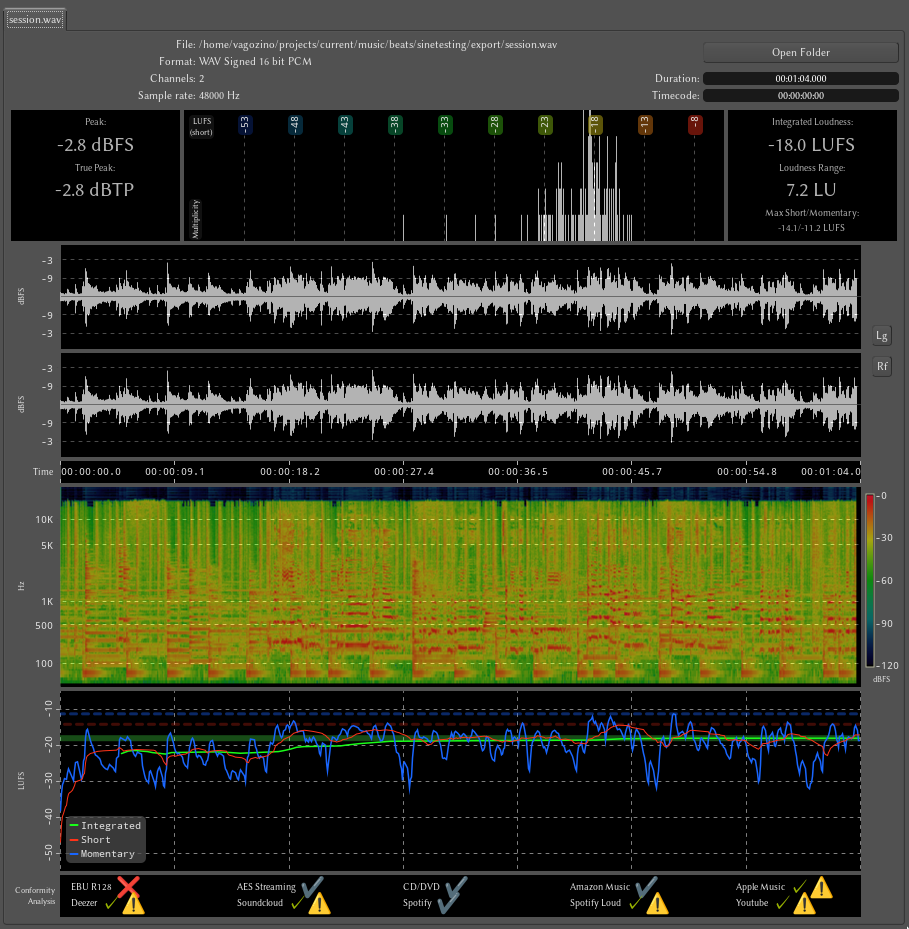
\includegraphics[width=\textwidth]{./assets/session.png}
    \caption{Ανάλυση του αρχείο \src{BringMetTheDiscoKing.wav} χωρίς εφαρμογή του \en{plugin}.}
    \label{fig:sessionanalysis}
\end{figure}

\begin{figure}[!h]
    \centering
    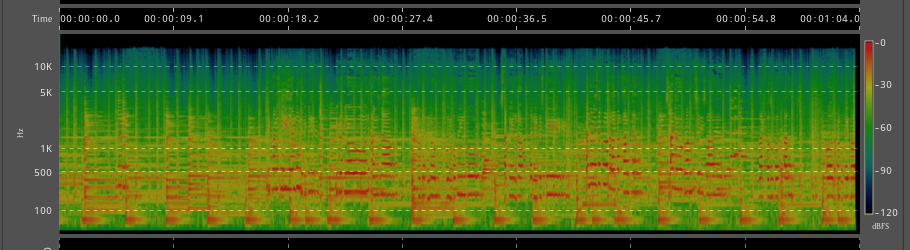
\includegraphics[width=\textwidth]{./assets/session_1000_lp.png}
    \caption{Ανάλυση του αρχείο \src{BringMetTheDiscoKing.wav} με εφαρμογή χαμηλοπερατού φίλτρου στα $1000Hz$.}
    \label{fig:sessionanalysislp1000}
\end{figure}

\begin{figure}[H]
    \centering
    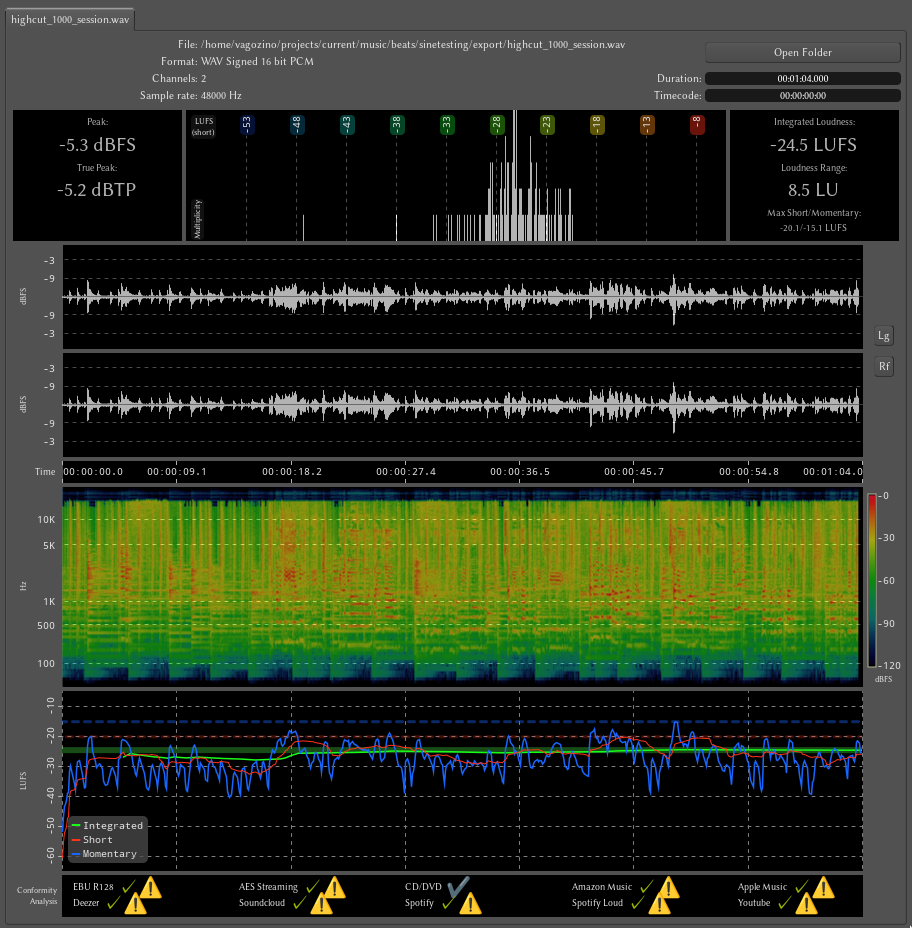
\includegraphics[width=\textwidth]{./assets/session_1000_hp.png}
    \caption{Ανάλυση του αρχείο \src{BringMetTheDiscoKing.wav} με εφαρμογή υψιπερατού φίλτρου στα $1000Hz$.}
    \label{fig:sessionanalysishp1000}
\end{figure}

Μπορούμε από τις μετρήσεις να επιβεβαιώσουμε τη σωστή λειτουργία του φίλτρου. Σαφώς, η σωστή 
λειτουργία ενός \en{plugin} κρίνεται πληρέστερα από την μεριά του χρήστη. Στο μέλλον
θα θέλαμε να παρουσιάσουμε το εργαλείο σε χρήστες ώστε να έχουμε μία εικόνα πάνω 
στην ευχρηστεία και την ποιότητα της επεξεργασίας του.

\section{Συμπεράσματα}

Η χρήση μίας βιβλιοθήκης όπως η \en{JUCE} φέρνει πολλά χρήσιμα εργαλεία 
αφού διαχωρίζει την ανάπτυξη του \en{DSP} από την λειτουργεία του συστήματος που 
θα φιλοξενήσει το \en{plugin}. 

Ένα σύγχρονο σύστημα αποτελείται από πολλά κινούμενα μέρη, από τις εφαρμογές 
του μέχρι την τελική επικοινωνία με το υλικό. Όλα αυτά συνδέονται μεταξύ τους
με (επί το πλείστον) συμπαγείς αφαιρέσεις όπως είναι ο διακοσμιτής ήχου (\en{sound server}).
Για την καλύτερη κατανόηση των προκλήσεων ανάπτυξης μιας τέτοιας εφαρμογής είναι χρήσιμη  η
παρουσίαση όλων αυτών των κομματιών.

Η τεχνολογία των \en{Audio Plugin Hosts} απλοποιεί πολύ 
τη χρήση των εφαρμογών μας αφού περίπλοκες πράξεις όπως ανακατεύθυνση της 
ροής ήχου από μία συσκευή σε μία άλλη μετατρέπεται στην γραφική σύνδεση
δύο νοητών θυρών με ένα νοητό καλώδιο.

Το τελικό εργαλείο που αναπτύξαμε στα πλαίσια της εργασίας είναι ένας απλοϊκός ισοσταθμιστής
ήχου. Οι επιδώσεις του είναι ικανοποιητικές αφού μπορεί να λειτουργήσει σε συνθήκες πραγματικού 
χρόνου χωρίς να υπάρχει επιβάρυνση στο σύστημα \say{οικοδεσπότη}. Επίσης, συνοδεύεται 
από μία ξεκάθαρη γραφική διεπαφή η οποία είναι πλήρως αποκομμένη από την εσωτερική λειτουργία
του \en{plugin}.

\newpage

\bibliography{bibliography}

\appendix

\section{Πηγαίος Κώδικας της Εφαρμογής}

Οι βασικοί φάκελοι της εφαρμογής είναι

\begin{itemize}
    \item \src{Builds} -- Τα εκτελέσιμα αρχεία.
    \item \src{Docs} -- Τεκμηρίωση της εργασίας.
    \item \src{JuceLibraryCode} -- Κώδικας βιβλιοθηκών του πακέτου \en{JUCE}.
    \item \src{Source} -- Ο πηγαίος κώδικας της εφαρμογής μας.
\end{itemize}

Ο κώδικας μπορεί να βρεθεί στο αποθετήριο: \en{\url{https://github.com/vagos/soundtechreport}}.

Οδηγίες χτησίματος της βιβλιοθήκης για κάθε πλατφόρμα μπορεί να βρεθεί στην τεκμηρίωση του πακέτου \en{JUCE}.

\end{document}
